 The concepts and notation in this section follow the treatments in~\cite{pierce1991basic,barr1990category}.

\begin{definition}
    \label{def:cat}
    A \textbf{category} is an unlabeled graph \( C \) together with a total function \( u : V(C) \to E(C) \) and a partial function \( \star: E(C) \times E(C) \to E(C) \) such that 
        \begin{itemize}
            \item for all edges \( f:X \to Y \) and \( g:Y \to Z \), the edge \( f \star g :X \to Z \) is defined; 
            \item  for every node \( X \), \( u(X) \) is an edge from \( X \) to \( X \);
            \item for every \( f:X \to Y \), we have \(u(X) \star f = f = f \star u(Y)\);
            \item for all edges \( f \), \( g \) and \(h\), we have \( (f \star g) \star h = f \star (g \star h) \) whenever either side is defined.
        \end{itemize}
    Edges are called \textbf{morphisms}. The function $\star$ is called \textbf{composition}. For all \( X \in V(C) \), the edge \( u(X) \) is denoted by \( \operatorname{id}_X \) and is called the \textbf{identity} of the object \( X \).
    % \( C \) is called the \textbf{underlying graph} of the category \( \mathcal{C} \).
\end{definition} 
\begin{definition}
    A category \(\mathcal{C}\) is said to be \textbf{locally small} if for all objects \(X,Y\) in \(\mathcal{C}\), the collection $\opn{Hom}(X,Y)$ of morphisms from \(X\) to \(Y\) is a set (called a \textbf{hom-set}). For a locally small category, $\opn{Mono}(X,Y)$ denotes the set of all monomorphisms from $X$ to $Y$.
\end{definition}
 Throughout this section, we fix a locally small category \( \mathcal{C} \).
\begin{example}
    Consider the unlabeled graph shown in~\autoref{fig:preliminaries:category}. 
        \begin{figure}[H]
        \centering
        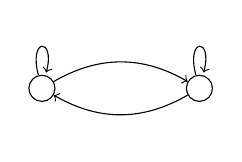
\begin{tikzpicture}
            \graphbox{}{0mm}{0mm}{32mm}{16mm}{-10mm}{-8mm}{
                \node[draw,circle] (1) at (0,0) {};
                \node[draw,circle] (2) at (2,0) {};
                \draw[->] (1) edge[loop above] node[midway, above] { } (1) ;
                \draw[->] (2) edge[loop above] node[midway, above] { } (2) ;
                \draw[->] (1) edge[bend left] node[midway, above] {}  (2)  ;
                \draw[->] (2) edge[bend left] node[midway, below] {} (1)   ;
            }
        \end{tikzpicture}
        \caption{}
        \label{fig:preliminaries:category}
    \end{figure}
    It can be considered as a category where the objects are the nodes and the morphisms are the paths between nodes; composition is path concatenation. The identity of a node is the self-loop of the node. There are at least three morphisms from the left node to itself: the identity morphism (the self-loop), the path that traverses the self-loop twice, and the path that goes to the right node and back.
\end{example}

% cat notation * 
\begin{notation}
    The composition of morphisms \( f : X \to Y \) and \( g : Y \to Z \) is written in diagrammatic order as \( f \star g \), rather than in functional order \( g \circ f \) as is common in litterature. The advantage is that, when reading from left to right, the morphisms appear in the same order as in the corresponding diagram, making the reasoning accompanying diagrams more intuitive. 
\end{notation}  

\begin{definition} 
    \label{def:cat:homo}
    A morphism \( f : X \to Y \) is said to be a \textbf{monomorphism} (is \textbf{monic}) if given any morphisms \( g,h: Z \to X  \), \( g \star f = h \star f \) implies \( g = h \). 
    In this case, we write $f : X \rightarrowtail Y$ to indicate that $f$ is a monomorphism.
\end{definition} 

\begin{example}
The category \(\mathbf{Set}\) has sets as objects and total functions between them as morphisms. For \(f\colon A\to B\) and \(g\colon B\to C\), composition is given by \(g\circ f\), and the identity morphism on a set \(A\) is the identity function \(\mathrm{id}_A\).
\end{example}

\begin{example} 
    Finite labeled graphs and their homomorphisms form a category, hereafter denoted by \textbf{Graph}. Its objects are labeled graphs, its morphisms are graph homomorphisms, and the monomorphisms are homomorphisms. 
    $\textbf{Graph}$ is locally small. 
\end{example}

% \begin{definition}[Span \cite{lowe2010graph}]
%     A pair \( (\alpha : A \to B,~\beta : A \to C) \) of morphisms with a common domain is called a \textbf{span}, denoted by \( B \overset{\alpha}{\leftarrow} A \overset{\beta}{\rightarrow} C \).
% \end{definition}
 
% \begin{definition}[Cospan]
%     A pair \( (\beta' : B \to D,~\alpha' : C \to D) \) of morphisms with a common codomain is called a \textbf{cospan}, denoted by \( B \overset{\beta'}{\rightarrow} D \overset{\alpha'}{\leftarrow} C \). 
% \end{definition} 
A span (resp. cospan) is a couple of morphisms with a common domain (resp. codomain).
\begin{definition}
An ordered pair \((\alpha : A \to B,\, \beta : A \to C)\) of morphisms with a common domain is called a \textbf{span} \cite{lowe2010graph}, denoted by
\(
B \overset{\alpha}{\leftarrow} A \overset{\beta}{\rightarrow} C
\). 
% An example of a span $(\alpha, \beta)$ is shown below.
Likewise, an ordered pair \((\beta' : B \to D,\, \alpha' : C \to D)\) of morphisms with a common codomain is called a \textbf{cospan}, denoted by
\(
B \overset{\beta'}{\rightarrow} D \overset{\alpha'}{\leftarrow} C
\). 
\end{definition}
\begin{example}
Consider the diagram in the category \textbf{Graph} shown in~\autoref{fig:preliminaries:span_cospan}. $(\alpha, \beta)$ is a span, and $(\beta', \alpha')$ is a cospan.
\end{example}


\begin{figure}[H]
   \centering
        \resizebox{0.7\textwidth}{!}{
        \begin{tikzpicture} 
            \graphbox{\( L \)}{40mm}{20mm}{34mm}{12mm}{2mm}{2mm}{
                \coordinate (o) at (0mm,-8mm); 
                \node[draw,circle] (l1) at ($(o)+(-10mm,0mm)$) {1};
                \node[draw,circle] (l2) at ($(l1)+(2,0)$) {2};
                \node[draw,circle,red] (l3) at ($(l1) + (1,0)$) {3};
                \draw[->,red] (l1) -- (l3) node[midway,above] {$a$};
                \draw[->,red] (l3) -- (l2) node[midway,above] {$a$};
            } 
    
            \graphbox{\( K \)}{0mm}{0mm}{34mm}{12mm}{2mm}{2mm}{
                \coordinate (o) at (0mm,-8mm); 
                \node[draw,circle] (l1) at ($(o)+(-10mm,0mm)$) {1};
                \node[draw,circle] (l2) at ($(l1)+(2,0)$) {2};
            }  
            \graphbox{\(G = L \cup C \)}{90mm}{5mm}{34mm}{27mm}{2mm}{-3mm}{
                \coordinate (o) at (0mm,-8mm); 
                \node[draw,circle] (l1) at ($(o)+(-10mm,0mm)$) {1};
                \node[draw,circle] (l2) at ($(l1)+(2,0)$) {2};
                \node[draw,circle,red] (l3) at ($(l1) + (1,0)$) {3};
                \node[draw,circle,blue] (l4) at ($(l2) + (0,-1)$) {6};
                \draw[->,red] (l1) -- (l3) node[midway,above] {$a$};
                \draw[->,red] (l3) -- (l2) node[midway,above] {$a$};
                \draw[->,blue] (l2) -- (l4) node[midway,right] {$a$};
                \node[draw,circle,blue] (l6) at ($(l1) + (0,-1)$) {7};
                \draw[<-,blue] (l1) -- (l6) node[midway,left] {$a$};
                \draw[->,blue] (l2) edge[out=-135,in=-45]node[midway,below] {$a$} (l1) ;
            }   
     
            \graphbox{\( C \)}{40mm}{-20mm}{34mm}{27mm}{2mm}{-3mm}{
                \coordinate (o) at (0mm,-8mm); 
                \node[draw,circle] (l1) at ($(o)+(-10mm,0mm)$) {1};
                \node[draw,circle] (l2) at ($(l1)+(2,0)$) {2};
                \node[draw,circle,blue] (l4) at ($(l2) + (0,-1)$) {6};
                \draw[->,blue] (l2) -- (l4) node[midway,right] {$a$};
                \draw[->,blue] (l2) edge[out=-135,in=-45]node[midway,below] {$a$} (l1) ;
                \node[ draw,circle,blue] (l6) at ($(l1) + (0,-1)$) {7};
                \draw[<-,blue] (l1) -- (l6) node[midway,left] {$a$};
            }      
            % K to L
            \draw[>->] (17mm,5mm) -- node[above] {$\alpha$} (37mm,15mm);
            % C to G
            \draw[>->] (76mm,-28mm)-- node[below] {$\alpha'$} (104mm,-24mm) ;
            % K to C
            \draw[>->] (17mm,-17mm) -- node[below] {$\beta$} (37mm,-28mm);
            % L to G
            \draw[>->] (76mm,16mm) -- node[above] {$\beta'$} (104mm,7mm);
            % \node () at (57mm,-6mm) {$PO$};
        \end{tikzpicture}
        }
        \caption{}
        \label{fig:preliminaries:span_cospan}
\end{figure}

\begin{definition}[\cite{barr1990category}]
    \label{def:cat:diagram}
    Let $\mathcal{C}$ be a category, and \( G \) an unlabeled graph. A \textbf{diagram} (of shape \( G \)) is a homomorphism of unlabeled graphs \( h : G \to \mathcal{C} \) where \( \mathcal{C} \) is considered as an unlabeled graph. A diagram is said to be \textbf{commutative} if, for all nodes \( u \), \( v \), and any two paths from \( u \) to \( v \) in the unlabeled graph \( G \):

    \begin{center}
    \resizebox{12cm}{!}{
        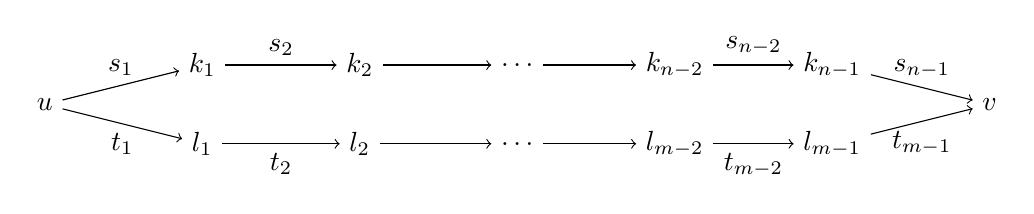
\begin{tikzpicture}
        \node (u) at (0,0) {\( u \)};
        \node (k1) at (2,0.5) {\( k_1 \)};
        \node (k2) at (4,0.5) {\( k_2 \)};
        \node (ketc) at (6,0.5) {\( \dots \)};
        \node (knm2) at (8,0.5) {\( k_{n-2} \)};
        \node (knm1) at (10,0.5) {\( k_{n-1} \)};
        \node (v) at (12,0) {\( v \)};
        \node (l1) at (2,-0.5) {\( l_1 \)};
        \node (l2) at (4,-0.5) {\( l_2 \)};
        \node (letc) at (6,-0.5) {\( \dots \)};
        \node (lnm2) at (8,-0.5) {\( l_{m-2} \)};
        \node (lnm1) at (10,-0.5) {\( l_{m-1} \)};
        \draw[->] (u) -- (k1) node [midway,above] {\( s_1 \)};
        \draw[->] (k1) -- (k2) node [midway,above] {\( s_2 \)};
        \draw[->] (k2) -- (ketc);
        \draw[->] (ketc) -- (knm2); 
        \draw[->] (knm2) -- (knm1) node[midway,above] {\( s_{n-2} \)}; 
        \draw[->] (knm1) -- (v) node[midway,above] {\( s_{n-1} \)}; 
        \draw[->] (u) -- (l1) node[midway,below] {\( t_1 \)};
        \draw[->] (l1) -- (l2) node[midway,below] {\( t_2 \)};
        \draw[->] (l2) -- (letc);
        \draw[->] (letc) -- (lnm2); 
        \draw[->] (lnm2) -- (lnm1) node[midway,below] {\( t_{m-2} \)}; 
        \draw[->] (lnm1) -- (v) node[midway,below] {\( t_{m-1} \)}; 
        \end{tikzpicture}
    }
    \end{center}
    \noindent
    the equality \( h(s_1) \star h(s_2) \star \dots  \star h(s_{n-1}) = h(t_1) \star h(t_2) \star \dots  \star h(t_{m-1}) \) holds.
\end{definition}

\begin{example}
    A commutative diagram in the category \textbf{Graph} of finite directed edge-labeled multigraphs is illustrated in~\autoref{fig:preliminaries:commutative_diagram}. The symbol $\mathop{=}$ in the center of the diagram
    is used to indicate that the two paths from node 1 to node 2 are equal.
 
    \begin{figure}[H]
        \centering
        \resizebox{0.7\textwidth}{!}{
        \begin{tikzpicture} 
            \graphbox{\( L \)}{40mm}{20mm}{34mm}{12mm}{2mm}{2mm}{
                \coordinate (o) at (0mm,-8mm); 
                \node[draw,circle] (l1) at ($(o)+(-10mm,0mm)$) {1};
                \node[draw,circle] (l2) at ($(l1)+(2,0)$) {2};
                \node[draw,circle,red] (l3) at ($(l1) + (1,0)$) {3};
                \draw[->,red] (l1) -- (l3) node[midway,above] {$a$};
                \draw[->,red] (l3) -- (l2) node[midway,above] {$a$};
            } 
    
            \graphbox{\( K \)}{0mm}{0mm}{34mm}{12mm}{2mm}{2mm}{
                \coordinate (o) at (0mm,-8mm); 
                \node[draw,circle] (l1) at ($(o)+(-10mm,0mm)$) {1};
                \node[draw,circle] (l2) at ($(l1)+(2,0)$) {2};
            }  
            \graphbox{\(G = L \cup C \)}{90mm}{5mm}{34mm}{27mm}{2mm}{-3mm}{
                \coordinate (o) at (0mm,-8mm); 
                \node[draw,circle] (l1) at ($(o)+(-10mm,0mm)$) {1};
                \node[draw,circle] (l2) at ($(l1)+(2,0)$) {2};
                \node[draw,circle,red] (l3) at ($(l1) + (1,0)$) {3};
                \node[draw,circle,blue] (l4) at ($(l2) + (0,-1)$) {6};
                \draw[->,red] (l1) -- (l3) node[midway,above] {$a$};
                \draw[->,red] (l3) -- (l2) node[midway,above] {$a$};
                \draw[->,blue] (l2) -- (l4) node[midway,right] {$a$};
                \node[draw,circle,blue] (l6) at ($(l1) + (0,-1)$) {7};
                \draw[<-,blue] (l1) -- (l6) node[midway,left] {$a$};
                \draw[->,blue] (l2) edge[out=-135,in=-45]node[midway,below] {$a$} (l1) ;
            }   
     
            \graphbox{\( C \)}{40mm}{-20mm}{34mm}{27mm}{2mm}{-3mm}{
                \coordinate (o) at (0mm,-8mm); 
                \node[draw,circle] (l1) at ($(o)+(-10mm,0mm)$) {1};
                \node[draw,circle] (l2) at ($(l1)+(2,0)$) {2};
                \node[draw,circle,blue] (l4) at ($(l2) + (0,-1)$) {6};
                \draw[->,blue] (l2) -- (l4) node[midway,right] {$a$};
                \draw[->,blue] (l2) edge[out=-135,in=-45]node[midway,below] {$a$} (l1) ;
                \node[ draw,circle,blue] (l6) at ($(l1) + (0,-1)$) {7};
                \draw[<-,blue] (l1) -- (l6) node[midway,left] {$a$};
            }      
            % K to L
            \draw[>->] (17mm,5mm) -- node[above] {$\alpha$} (37mm,15mm);
            % C to G
            \draw[>->] (76mm,-28mm)-- node[below] {$\alpha'$} (104mm,-24mm) ;
            % K to C
            \draw[>->] (17mm,-17mm) -- node[below] {$\beta$} (37mm,-28mm);
            % L to G
            \draw[>->] (76mm,16mm) -- node[above] {$\beta'$} (104mm,7mm);
            \node () at (57mm,-6mm) {$\mathop{=}$};
        \end{tikzpicture}
        }
        \caption{}
        \label{fig:preliminaries:commutative_diagram}
    \end{figure}
\end{example}

\begin{notation}
    When the context makes it clear, \( h_{AB} \) denotes a morphism \( h : A \to B \), and we refer to diagrams by listing their nodes, as is standard in geometry. 
    For example, we denote the diagram shown in \autoref{def:cat:po} by \( ACDB \) or \( ABDC \).
\end{notation}   

The pushout is a construction in category theory that can often be thought of as the construction of a new structure from two given structures by gluing them along a common interface structure.
\begin{definition}
    \label{def:cat:po} 
    A \textbf{pushout} of a span \( B \overset{\alpha}{\leftarrow} A \overset{\beta}{\rightarrow} C \), as shown in~\autoref{fig:preliminaries:pushout_sdfkjasdlgjfl}
    is defined as a cospan \( B \overset{\beta'}{\rightarrow} D \overset{\alpha'}{\leftarrow} C \) such that \( \alpha \star \beta' = \beta \star \alpha' \), and for every cospan \( B \overset{\gamma'}{\rightarrow} E \overset{\gamma}{\leftarrow} C \), if \( \alpha \star \gamma' = \beta \star \gamma \) holds, then there exists a unique morphism \(\delta : D \to E\) such that \( \gamma' = \beta' \star \delta \) and \( \gamma = \alpha' \star \delta \).
    \begin{figure}[H]
        \centering
        \resizebox{0.4\textwidth}{!}{
            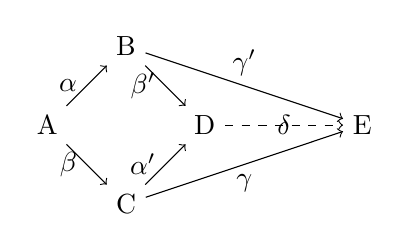
\begin{tikzpicture}
                    \node (i) at (0,0) {A};
                    \node (r) at (1,1) {B};
                    \node (c) at (1,-1) {C};
                    \node (h) at (2,0) {D};
                    % \node () at (1,-1) {\( \Delta \)};
                    \draw[->]  (i) -- (r) node [midway,left] {$ \alpha $};
                    \draw[->] (c) -- (h) node [midway,left] {$ \alpha' $};
                    \draw[->] (r) -- (h) node[midway, left] {$ \beta' $};
                    \draw[->] (i) -- (c) node[midway, left] {$ \beta $};
                    \node (d') at (4,0) {E};
                    \draw[->] (c) -- (d') node [midway,below]{$ \gamma $};
                    \draw[->] (r) -- (d') node [midway,above]{$ \gamma' $};
                    \draw[->,dashed] (h) -- (d') node [midway]{$ \delta $};
                \end{tikzpicture}
        }
        \caption{}
        \label{fig:preliminaries:pushout_sdfkjasdlgjfl}
    \end{figure}
The diagram involving \( (\alpha, \beta, \alpha', \beta') \) is called the \textbf{pushout square}, with \(D\) as the \textbf{pushout object}. The existence of a unique morphism is known as the \textbf{universal mapping property of the pushout}.
\end{definition} 

\begin{example}
    \label{ex:cat:posfjsdlkgja}
     Pushouts of two morphisms always exist in \(\mathbf{Set}\), and (up to isomorphism) can be described as follows. Let
    \( B \overset{\alpha}{\leftarrow} A \overset{\beta}{\rightarrow} C \) be a span. Its pushout is the cospan \( B \overset{\beta'}{\rightarrow} D \overset{\alpha'}{\leftarrow} C \) where the pushout object of \((\alpha,\beta)\) is the set
    \[
    D \;=\; (B + C)/{\sim}
    \]
    where \(B + C\) denotes the disjoint union of $B$ and $C$ and \(\sim\) is the smallest equivalence relation that includes \(\set{(\alpha(a),\beta(b))\mid a \in A }\). The maps
    \(\beta' \colon B\to D\) and \(\alpha' \colon C\to D\) send each element to its equivalence class.

    %  Consider the functions \(b\) and \(c\) shown in~\autoref{fig:preliminaries:a_rewriting_step_dfjalsdkjflg} in the category \(\mathbf{Set}\). Each set is drawn as a box; elements of a set are represented by circles. The numbers inside circles indicate how the functions map those elements. 
    %  The element labeled by $n$ in set $X$ is denoted by $n_X$ to avoid ambiguity.
    %  The equivalence relation \(\sim\) is the set \(\set{(1_B,1_C),(2_B,2_C)}\). The disjoint union of \(B\) and \(C\) is $D = \set{1_B,2_B,4_B,1_C,2_C,3_C}$. The quotient set $D/{\sim}$ is $\set{[1_B],[2_B],[3_C],[4_B]}$, where $[x]$ denotes the equivalence class of $x$. Note that $[1_C] = [1_B]$ and $[2_C] = [2_B]$, and $\set{[1_B],[2_B],[3_C],[4_B]}$ is isomorphic to $\set{1_D,2_D,3_D,4_D}$.
    For example, consider the functions \(\alpha\) and \(\beta\) shown in Figure~\ref{fig:preliminaries:a_rewriting_step_dfjalsdkjflg} in the category \(\mathbf{Set}\) where each set is drawn as a box and its elements are represented by circles. The numbers inside circles indicate how the functions map those elements.
    \begin{figure}[H]
      \centering 
      \resizebox{0.7\textwidth}{!}{
      \begin{tikzpicture}
          \graphbox{\( A\)}{40mm}{-3mm}{34mm}{12mm}{2mm}{2mm}{
              \coordinate (o) at (0mm,-8mm); 
              \node[draw,circle] (l1) at ($(o)+(-10mm,0mm)$) {1};
              \node[draw,circle] (l2) at ($(l1)+(2,0)$) {2};
          }  
          \graphbox{\( B \)}{80mm}{-3mm}{45mm}{12mm}{2mm}{2mm}{
              \coordinate (o) at (-5mm,-8mm); 
              \node[draw,circle] (l1) at ($(o)+(-10mm,0mm)$) {1};
              \node[draw,circle] (l2) at ($(l1)+(3,0)$) {2};
              \node[draw,circle] (l3) at ($(l1) + (1,0)$) {4};
            %   \node[draw,circle] (l4) at ($(l1) + (2,0)$) {5};
            %   \draw[ ] (l1) -- (l3) node[midway,above] {$a$};
            %   \draw[ ] (l3) -- (l4) node[midway,above] {$b$};
            %   \draw[ ] (l4) -- (l2) node[midway,above] {$a$};
          }     
          \graphbox{\( C  \)}{40mm}{-22mm}{34mm}{22mm}{2mm}{-3mm}{
              \coordinate (o) at (0mm,-3mm); 
              \node[draw,circle] (l1) at ($(o)+(-10mm,0mm)$) {1};
              \node[draw,circle] (l2) at ($(l1)+(2,0)$) {2};
            %   \node[draw,circle] (l4) at ($(l2) + (0,-1)$) {6};
              \node[ draw,circle] (l6) at ($(l1) + (0,-1)$) {3};
            %   \draw[ ] (l1) -- (l6) node[midway,left] {$a$};
            %   \draw[ ] (l2) -- (l4) node[midway,right] {$a$};
          }    
          \graphbox{\( D \)}{80mm}{-22mm}{45mm}{22mm}{2mm}{-3mm}{
              \coordinate (o) at (-5mm,-3mm); 
              \node[draw,circle] (l1) at ($(o)+(-10mm,0mm)$) {1};
              \node[draw,circle] (l2) at ($(l1)+(3,0)$) {2};
              \node[draw,circle] (l3) at ($(l1) + (1,0)$) {4};
            %   \node[draw,circle] (l4) at ($(l1) + (2,0)$) {5};
            %   \node[ draw,circle] (l5) at ($(l2) + (0,-1)$) {6};
              \node[ draw,circle] (l6) at ($(l1) + (0,-1)$) {3};
            %   \draw[ ] (l1) -- (l6) node[midway,left] {$a$};
            %   \draw[] (l1) -- (l3) node[midway,above] {$a$};
            %   \draw[] (l3) -- (l4) node[midway,above] {$b$};
            %   \draw[ ] (l4) -- (l2) node[midway,above] {$a$};
            %   \draw[ ] (l2) -- (l5) node[midway,right] {$a$};
          }    
          \node () at (77mm,-8mm) {\( \overset{\alpha}{\rightarrowtail} \)}; % K -> R
          \node () at (58mm,-18mm) {\( \beta\downarrowtail \)};
          \node () at (102mm,-18mm) {\( \beta'\downarrowtail \)};
          \node () at (77mm,-33mm) {\( \overset{\alpha'}{\rightarrowtail} \)}; % C -> H
      \end{tikzpicture}
      }
      \caption{}
      \label{fig:preliminaries:a_rewriting_step_dfjalsdkjflg}
  \end{figure}
    Throughout this example, an element labeled \(n\) in a set \(X\) is denoted by \(n_X\) to avoid ambiguity.        
    The binary relation \(\sim\) is the reflexive, symmetric and transitive closure of the binary relation $\{(1_B,1_C),(2_B,2_C)\}$.
 
    The disjoint union of \(B\) and \(C\) is
    \[ 
    D' = \{1_B,2_B,4_B,1_C,2_C,3_C\},
    \]
    and the quotient \(D'/\sim\) is
    \[
    D'/\sim = \{[1_B],[2_B],[3_C],[4_B]\},
    \]
    We have \([1_C]=[1_B]\) and \([2_C]=[2_B]\), and the maps
    \(\beta'' \colon B\to D'\) and \(\alpha'' \colon C\to D'\) send each element to its equivalence class. Note that \(\{[1_B],[2_B],[3_C],[4_B]\}\) is isomorphic to \(D\), shown in \autoref{fig:preliminaries:a_rewriting_step_dfjalsdkjflg}, which is expected because the pushout of a span is unique up to isomorphism.
\end{example}

\begin{proposition}{\cite{corradini1997algebraic}[p.188]}
    \label{prop:pushout_graph_always_exists}
    In category \textbf{Graph} the pushout of two arrows always exists: It can be computed componentwise (as a pushout in \textbf{Set}) for the nodes and for the edges, and the source, target, and labeling mappings are uniquely determined.
\end{proposition}

\begin{example}
    The diagram in~\autoref{fig:preliminaries:pushout_injective} is a pushout square in the category \textbf{Graph}. In this example, both $\alpha$ and $\beta$ are injective morphisms. Therefore, the pushout object $G$ can be constructed easily by taking the interface graph $K$ and adding elements from $L$ and $C$ which are not present in $K$.
    \begin{figure}[H]
        \centering
        \resizebox{0.7\textwidth}{!}{
        \begin{tikzpicture} 
            \graphbox{\( L \)}{40mm}{20mm}{34mm}{12mm}{2mm}{2mm}{
                \coordinate (o) at (0mm,-8mm); 
                \node[draw,circle] (l1) at ($(o)+(-10mm,0mm)$) {1};
                \node[draw,circle] (l2) at ($(l1)+(2,0)$) {2};
                \node[draw,circle,red] (l3) at ($(l1) + (1,0)$) {3};
                \draw[->,red] (l1) -- (l3) node[midway,above] {$a$};
                \draw[->,red] (l3) -- (l2) node[midway,above] {$a$};
            } 
    
            \graphbox{\( K \)}{0mm}{0mm}{34mm}{12mm}{2mm}{2mm}{
                \coordinate (o) at (0mm,-8mm); 
                \node[draw,circle] (l1) at ($(o)+(-10mm,0mm)$) {1};
                \node[draw,circle] (l2) at ($(l1)+(2,0)$) {2};
            }  
            \graphbox{\(G  \)}{90mm}{5mm}{34mm}{27mm}{2mm}{-3mm}{
                \coordinate (o) at (0mm,-8mm); 
                \node[draw,circle] (l1) at ($(o)+(-10mm,0mm)$) {1};
                \node[draw,circle] (l2) at ($(l1)+(2,0)$) {2};
                \node[draw,circle,red] (l3) at ($(l1) + (1,0)$) {3};
                \node[draw,circle,blue] (l4) at ($(l2) + (0,-1)$) {6};
                \draw[->,red] (l1) -- (l3) node[midway,above] {$a$};
                \draw[->,red] (l3) -- (l2) node[midway,above] {$a$};
                \draw[->,blue] (l2) -- (l4) node[midway,right] {$a$};
                \node[draw,circle,blue] (l6) at ($(l1) + (0,-1)$) {7};
                \draw[<-,blue] (l1) -- (l6) node[midway,left] {$a$};
                \draw[->,blue] (l2) edge[out=-135,in=-45]node[midway,below] {$a$} (l1) ;
            }   
     
            \graphbox{\( C \)}{40mm}{-20mm}{34mm}{27mm}{2mm}{-3mm}{
                \coordinate (o) at (0mm,-8mm); 
                \node[draw,circle] (l1) at ($(o)+(-10mm,0mm)$) {1};
                \node[draw,circle] (l2) at ($(l1)+(2,0)$) {2};
                \node[draw,circle,blue] (l4) at ($(l2) + (0,-1)$) {6};
                \draw[->,blue] (l2) -- (l4) node[midway,right] {$a$};
                \draw[->,blue] (l2) edge[out=-135,in=-45]node[midway,below] {$a$} (l1) ;
                \node[ draw,circle,blue] (l6) at ($(l1) + (0,-1)$) {7};
                \draw[<-,blue] (l1) -- (l6) node[midway,left] {$a$};
            }      
            % K to L
            \draw[>->] (17mm,5mm) -- node[above] {$\alpha$} (37mm,15mm);
            % C to G
            \draw[>->] (76mm,-28mm)-- node[below] {$\alpha'$} (104mm,-24mm) ;
            % K to C
            \draw[>->] (17mm,-17mm) -- node[below] {$\beta$} (37mm,-28mm);
            % L to G
            \draw[>->] (76mm,16mm) -- node[above] {$\beta'$} (104mm,7mm);
            \node () at (57mm,-6mm) {$PO$};
        \end{tikzpicture}
        }
        \caption{Pushout square with injective morphisms.}
        \label{fig:preliminaries:pushout_injective}
    \end{figure}
\end{example}

\begin{example}
    The diagram in~\autoref{fig:preliminaries:pushout_non_injective} is a pushout square in the category \textbf{Graph}. In this example, $\beta$ is not injective. Therefore, some elements are merged in the pushout object $G$.

    \begin{figure}[H]
        \centering 
        \resizebox{0.7\textwidth}{!}{
        \begin{tikzpicture} 
            \graphbox{\( L \)}{40mm}{20mm}{34mm}{20mm}{2mm}{2mm}{
                \coordinate (o) at (0mm,-8mm); 
                \node[draw,circle] (l1) at ($(o)+(-10mm,0mm)$) {1};
                \node[draw,circle] (l2) at ($(l1)+(2,0)$) {2};
                \draw[->,red] (l2) edge[out=-135,in=-45]node[midway,below] {$a$} (l1) ;
                \node[draw,circle,red] (l3) at ($(l1) + (1,0)$) {3};
                \draw[->,red] (l1) -- (l3) node[midway,above] {$a$};
                \draw[->,red] (l3) -- (l2) node[midway,above] {$a$};
            } 
    
            \graphbox{\( K \)}{0mm}{0mm}{34mm}{12mm}{2mm}{2mm}{
                \coordinate (o) at (0mm,-8mm); 
                \node[draw,circle] (l1) at ($(o)+(-10mm,0mm)$) {1};
                \node[draw,circle] (l2) at ($(l1)+(2,0)$) {2};
            }  
            \graphbox{\(G  \)}{110mm}{5mm}{34mm}{40mm}{2mm}{-3mm}{
                \coordinate (o) at (0mm,-20mm); 
                 \node[draw,circle] (l1) at ($(o)+(0,0)$) {1\ 2};
                % \node[draw,circle] (l1) at ($(o)+(-10mm,0mm)$) {1};
                % \node[draw,circle] (l2) at ($(l1)+(2,0)$) {2};
                \draw[->,red] (l1) edge[loop below] node[midway, below] {$a$} (l1) ;
                \node[draw,circle,red] (l3) at ($(l1) + (0,1.4)$) {3};
                \node[draw,circle,blue] (l4) at ($(l1) + (1,-1)$) {6};
                \draw[->,red] (l1) edge[bend left] node[midway,left] {$a$} (l3);
                \draw[->,red] (l3) edge[bend left] node[midway,right] {$a$} (l1);
                \draw[->,blue] (l1) edge  node[midway,right] {$a$} (l4);
                \node[draw,circle,blue] (l6) at ($(l1) + (-1,-1)$) {7};
                \draw[<-,blue] (l1) edge node[midway,left] {$a$} (l6) ;
                % \draw[->,blue] (l1) edge[out=-135,in=-45]node[midway,below] {$a$} (l1) ;
            }   
     
            \graphbox{\( C \)}{40mm}{-20mm}{34mm}{35mm}{2mm}{-3mm}{
                \coordinate (o) at (0mm,-14mm); 
                \node[draw,circle] (l1) at ($(o)+(0,0)$) {1\ 2};
                % \node[draw,circle] (l2) at ($(l1)+(2,0)$) {2};
                \node[draw,circle,blue] (l4) at ($(l1) + (1,-1)$) {6};
                \draw[->,blue] (l1) -- (l4) node[midway,right] {$a$};
                % \draw[->,blue] (l1) edge[loop above] node[midway, above] {$a$} (l1) ;
                \node[ draw,circle,blue] (l6) at ($(l1) + (-1,-1)$) {7};
                \draw[<-,blue] (l1) -- (l6) node[midway,left] {$a$};
            }
            % K to L  
            \draw[>->] (17mm,5mm) -- node[above] {$\alpha$} (37mm,15mm);
            % C to G
            \draw[>->] (76mm,-28mm)-- node[below] {$\alpha'$} (104mm,-24mm) ;
            % K to C
            \draw[->] (17mm,-17mm) -- node[below] {$\beta$} (37mm,-28mm);
            % L to G
            \draw[->] (76mm,16mm) -- node[above] {$\beta'$} (104mm,7mm);
            \node () at (57mm,-6mm) {$PO$};
        \end{tikzpicture}
        }
        \caption{Pushout square with a non-injective morphism.}
        \label{fig:preliminaries:pushout_non_injective}
    \end{figure} 
\end{example}
The \emph{pullback}, defined below, is the dual construction of the pushout in category theory, and it can be thought of as construction of the interface structure along which two structures are glued together. 
\begin{definition} 
    \label{def:cat:pb}
   A \textbf{pullback} of a cospan \(B \overset{\beta'}{\rightarrow} D \overset{\alpha'}{\leftarrow} C \), as shown in~\autoref{fig:preliminaries:pullback_ssdsfd},
is a span \( B \overset{\alpha}{\leftarrow} A \overset{\beta}{\rightarrow} C \) such that \( \alpha \star \beta' = \beta \star \alpha' \), and for every span \( B \overset{\gamma'}{\leftarrow} E \overset{\gamma}{\rightarrow} C \) if \(\gamma' \star \beta' = \gamma \star \alpha'\) holds, then there exists a unique morphism \(\delta: E \to A\) such that $\gamma' = \delta \star \alpha$ and $\gamma = \delta \star \beta$. 
    \begin{figure}[H]
        \centering  
        \resizebox{0.4\textwidth}{!}{
                    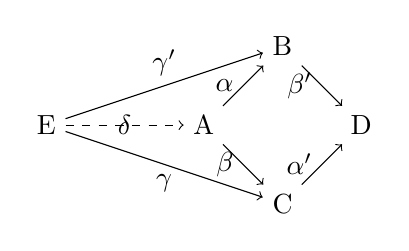
\begin{tikzpicture}
                        \node (i) at (0,0) {A};
                        \node (r) at (1,1) {B};
                        \node (c) at (1,-1) {C};
                        \node (h) at (2,0) {D}; 
                        % \node () at (1,-1) {\( \Delta \)};
                        \draw[->]  (i) -- (r) node [midway,left] {$\alpha$};
                        \draw[->] (c) -- (h) node [midway,left] {$\alpha'$};
                        \draw[->] (r) -- (h) node[midway, left] {$\beta'$};
                        \draw[->] (i) -- (c) node[midway, left] {$\beta$};
                        \node (d') at (-2,0) {E};
                        \draw[<-] (c) -- (d') node [midway,below]{$\gamma$};
                        \draw[<-] (r) -- (d') node [midway,above]{$\gamma'$};
                        \draw[->, dashed] (d') -- (i) node [midway]{$\delta$};
                    \end{tikzpicture}
        }
        \caption{}
        \label{fig:preliminaries:pullback_ssdsfd}
    \end{figure}
The diagram involving \( (\alpha, \beta, \alpha', \beta') \) is called the \textbf{pullback square}, with \(A\) as the \textbf{pullback object}. The existence of a unique morphism is known as the \textbf{universal mapping property of the pullback}.
\end{definition} 
In the category \textbf{Graph} pullbacks always exist and are computed pointwise: take the pullback in \textbf{Set} of the node sets and of the edge sets, and equip the resulting graph with source, target and labeling maps induced componentwise; the projection graph homomorphisms are the corresponding componentwise projections and satisfy the universal property.
\begin{example} 
    In the category \textbf{Set},
    the pullback 
    of a cospan \(B \overset{\beta'}{\rightarrow} D \overset{\alpha'}{\leftarrow} C \) is the span \( B \overset{\alpha}{\leftarrow} A \overset{\beta}{\rightarrow} C \) where
    the pullback object $A$ is the set $A = \set{(b,c) \mid \beta (c) = \alpha (b)} \subseteq B \times C$; $\alpha$ and $\beta$ are defined as the corresponding projections, e.g., $\alpha((b, c)) = b$ and $\beta((b, c)) = c$.

    Consider the cospan \(B \overset{\beta'}{\rightarrow} D \overset{\alpha'}{\leftarrow} C \) shown in~\autoref{fig:preliminaries:a_rewriting_step_dfjalsdkdfsdfjflg}. 
    The span \( B \overset{\alpha}{\leftarrow} A \overset{\beta}{\rightarrow} C \) shown in~\autoref{fig:preliminaries:a_rewriting_step_dfjalsdkdfsdfjflg} is the pullback of this cospan.
    Indeed, the pullback object can be taken as the set $A' = \set{(1_B,1_C),(2_B,2_C)} \subseteq B \times C$, and the morphisms $\alpha'' \colon A' \to B$ and $\beta'' \colon A' \to C$ are defined as the corresponding projections, e.g., $\alpha''((x,y)) = x$ and $\beta''((x,y)) = y$. Note that $A$ is isomorphic to $A'$, which is expected because the pullback of a cospan is unique up to isomorphism.
      \begin{figure}[H]
      \centering 
      \resizebox{0.7\textwidth}{!}{
      \begin{tikzpicture}
          \graphbox{\( A\)}{40mm}{-3mm}{34mm}{12mm}{2mm}{2mm}{
              \coordinate (o) at (0mm,-8mm); 
              \node[draw,circle] (l1) at ($(o)+(-10mm,0mm)$) {1};
              \node[draw,circle] (l2) at ($(l1)+(2,0)$) {2};
          }  
          \graphbox{\( B \)}{80mm}{-3mm}{45mm}{12mm}{2mm}{2mm}{
              \coordinate (o) at (-5mm,-8mm); 
              \node[draw,circle] (l1) at ($(o)+(-10mm,0mm)$) {1};
              \node[draw,circle] (l2) at ($(l1)+(3,0)$) {2};
              \node[draw,circle] (l3) at ($(l1) + (1,0)$) {4};
            %   \node[draw,circle] (l4) at ($(l1) + (2,0)$) {5};
            %   \draw[ ] (l1) -- (l3) node[midway,above] {$a$};
            %   \draw[ ] (l3) -- (l4) node[midway,above] {$b$};
            %   \draw[ ] (l4) -- (l2) node[midway,above] {$a$};
          }     
          \graphbox{\( C  \)}{40mm}{-22mm}{34mm}{22mm}{2mm}{-3mm}{
              \coordinate (o) at (0mm,-3mm); 
              \node[draw,circle] (l1) at ($(o)+(-10mm,0mm)$) {1};
              \node[draw,circle] (l2) at ($(l1)+(2,0)$) {2};
            %   \node[draw,circle] (l4) at ($(l2) + (0,-1)$) {6};
              \node[ draw,circle] (l6) at ($(l1) + (0,-1)$) {3};
            %   \draw[ ] (l1) -- (l6) node[midway,left] {$a$};
            %   \draw[ ] (l2) -- (l4) node[midway,right] {$a$};
          }    
          \graphbox{\( D \)}{80mm}{-22mm}{45mm}{22mm}{2mm}{-3mm}{
              \coordinate (o) at (-5mm,-3mm); 
              \node[draw,circle] (l1) at ($(o)+(-10mm,0mm)$) {1};
              \node[draw,circle] (l2) at ($(l1)+(3,0)$) {2};
              \node[draw,circle] (l3) at ($(l1) + (1,0)$) {4};
            %   \node[draw,circle] (l4) at ($(l1) + (2,0)$) {5};
            %   \node[ draw,circle] (l5) at ($(l2) + (0,-1)$) {6};
              \node[ draw,circle] (l6) at ($(l1) + (0,-1)$) {3};
            %   \draw[ ] (l1) -- (l6) node[midway,left] {$a$};
            %   \draw[] (l1) -- (l3) node[midway,above] {$a$};
            %   \draw[] (l3) -- (l4) node[midway,above] {$b$};
            %   \draw[ ] (l4) -- (l2) node[midway,above] {$a$};
            %   \draw[ ] (l2) -- (l5) node[midway,right] {$a$};
          }    
          \node () at (77mm,-8mm) {\( \overset{\alpha}{\rightarrowtail} \)};
          \node () at (58mm,-18mm) {\( \beta\downarrowtail \)};
          \node () at (102mm,-18mm) {\( \beta'\downarrowtail \)};
          \node () at (77mm,-33mm) {\( \overset{\alpha'}{\rightarrowtail} \)};
      \end{tikzpicture}
      }
      \caption{}
      \label{fig:preliminaries:a_rewriting_step_dfjalsdkdfsdfjflg}
  \end{figure}
\end{example}

\begin{example}
    Consider the diagram shown in~\autoref{fig:preliminaries:pullback} in the category \textbf{Graph}.
    The span $L \overset{\alpha}{\leftarrow} K \overset{\beta}{\rightarrow} C$ is a pullback of the cospan $L \overset{\beta'}{\rightarrow} G \overset{\alpha'}{\leftarrow} C$.
    \begin{figure}[H]
        \centering
        \resizebox{0.9\textwidth}{!}{
        \begin{tikzpicture} 
            \graphbox{\( L \)}{40mm}{20mm}{34mm}{20mm}{2mm}{2mm}{
                \coordinate (o) at (0mm,-8mm); 
                \node[draw,circle] (l1) at ($(o)+(-10mm,0mm)$) {1};
                \node[draw,circle] (l2) at ($(l1)+(2,0)$) {2};
                \draw[->,red] (l2) edge[out=-135,in=-45]node[midway,below] {$a$} (l1) ;
                \node[draw,circle,red] (l3) at ($(l1) + (1,0)$) {3};
                \draw[->,red] (l1) -- (l3) node[midway,above] {$a$};
                \draw[->,red] (l3) -- (l2) node[midway,above] {$a$};
            } 
    
            \graphbox{\( K \)}{0mm}{0mm}{34mm}{12mm}{2mm}{2mm}{
                \coordinate (o) at (0mm,-8mm); 
                \node[draw,circle] (l1) at ($(o)+(-10mm,0mm)$) {1};
                \node[draw,circle] (l2) at ($(l1)+(2,0)$) {2};
            }  
            \graphbox{\(G  \)}{110mm}{5mm}{34mm}{40mm}{2mm}{-3mm}{
                \coordinate (o) at (0mm,-20mm); 
                 \node[draw,circle] (l1) at ($(o)+(0,0)$) {1\ 2};
                % \node[draw,circle] (l1) at ($(o)+(-10mm,0mm)$) {1};
                % \node[draw,circle] (l2) at ($(l1)+(2,0)$) {2};
                \draw[->,red] (l1) edge[loop below] node[midway, below] {$a$} (l1) ;
                \node[draw,circle,red] (l3) at ($(l1) + (0,1.4)$) {3};
                \node[draw,circle,blue] (l4) at ($(l1) + (1,-1)$) {6};
                \draw[->,red] (l1) edge[bend left] node[midway,left] {$a$} (l3);
                \draw[->,red] (l3) edge[bend left] node[midway,right] {$a$} (l1);
                \draw[->,blue] (l1) edge  node[midway,right] {$a$} (l4);
                \node[draw,circle,blue] (l6) at ($(l1) + (-1,-1)$) {7};
                \draw[<-,blue] (l1) edge node[midway,left] {$a$} (l6) ;
                % \draw[->,blue] (l1) edge[out=-135,in=-45]node[midway,below] {$a$} (l1) ;
            }   
     
            \graphbox{\( C \)}{40mm}{-20mm}{34mm}{35mm}{2mm}{-3mm}{
                \coordinate (o) at (0mm,-14mm); 
                \node[draw,circle] (l1) at ($(o)+(0,0)$) {1\ 2};
                % \node[draw,circle] (l2) at ($(l1)+(2,0)$) {2};
                \node[draw,circle,blue] (l4) at ($(l1) + (1,-1)$) {6};
                \draw[->,blue] (l1) -- (l4) node[midway,right] {$a$};
                % \draw[->,blue] (l1) edge[loop above] node[midway, above] {$a$} (l1) ;
                \node[ draw,circle,blue] (l6) at ($(l1) + (-1,-1)$) {7};
                \draw[<-,blue] (l1) -- (l6) node[midway,left] {$a$};
            }
            % K to L  
            \draw[>->] (17mm,5mm) -- node[above] {$\alpha$} (37mm,15mm);
            % C to G
            \draw[>->] (76mm,-28mm)-- node[below] {$\alpha'$} (104mm,-24mm) ;
            % K to C
            \draw[->] (17mm,-17mm) -- node[below] {$\beta$} (37mm,-28mm);
            % L to G 
            \draw[->] (76mm,16mm) -- node[above] {$\beta'$} (104mm,7mm);
            \node () at (57mm,-6mm) {$PB$};
        \end{tikzpicture}
        }
        \caption{Pullback.}
        \label{fig:preliminaries:pullback}
    \end{figure} 

 
    % Specifically, for a possible span \( B \overset{\gamma'}{\leftarrow} E \overset{\gamma}{\rightarrow} C \) to satisfy \(\gamma' \star \beta' = \gamma \star \alpha'\), graph $E$ must not contain any edges as $\alpha'$ and $\beta'$ do not map any edges from $C$ and $L$ to a common edge in $G$.
    %  For all graph $E$ without edges and all morphisms $\gamma': E \rightarrow L $ and $\gamma : E \rightarrow C$, we have \(\gamma' \star \beta' = \gamma \star \alpha'\). Three examples of such spans are illustrated in~\autoref{fig:preliminaries:three_squares}.
    % \begin{figure}[H]
    %     \centering
    %         \resizebox{0.7\textwidth}{!}{
    %         \begin{tikzpicture} 
    %             \graphbox{\( E_1 \)}{-50mm}{0mm}{34mm}{12mm}{2mm}{2mm}{
    %                 \coordinate (o) at (0mm,-8mm); 
    %                 \node[draw,circle] (l1) at ($(o)+(-10mm,0mm)$) {1};
    %                 \node[draw,circle] (l2) at ($(l1)+(2,0)$) {2};
    %             }  
    %             \graphbox{\( L \)}{40mm}{20mm}{34mm}{20mm}{2mm}{2mm}{
    %                 \coordinate (o) at (0mm,-8mm); 
    %                 \node[draw,circle] (l1) at ($(o)+(-10mm,0mm)$) {1};
    %                 \node[draw,circle] (l2) at ($(l1)+(2,0)$) {2};
    %                 \draw[->,red] (l2) edge[out=-135,in=-45]node[midway,below] {$a$} (l1) ;
    %                 \node[draw,circle,red] (l3) at ($(l1) + (1,0)$) {3};
    %                 \draw[->,red] (l1) -- (l3) node[midway,above] {$a$};
    %                 \draw[->,red] (l3) -- (l2) node[midway,above] {$a$};
    %             } 
        
    %             \graphbox{\( K \)}{0mm}{0mm}{34mm}{12mm}{2mm}{2mm}{
    %                 \coordinate (o) at (0mm,-8mm); 
    %                 \node[draw,circle] (l1) at ($(o)+(-10mm,0mm)$) {1};
    %                 \node[draw,circle] (l2) at ($(l1)+(2,0)$) {2};
    %             }  

    %             \graphbox{\( C \)}{40mm}{-20mm}{34mm}{35mm}{2mm}{-3mm}{
    %                 \coordinate (o) at (0mm,-14mm); 
    %                 \node[draw,circle] (l1) at ($(o)+(0,0)$) {1\ 2};
    %                 % \node[draw,circle] (l2) at ($(l1)+(2,0)$) {2};
    %                 \node[draw,circle,blue] (l4) at ($(l1) + (1,-1)$) {6};
    %                 \draw[->,blue] (l1) -- (l4) node[midway,right] {$a$};
    %                 % \draw[->,blue] (l1) edge[loop above] node[midway, above] {$a$} (l1) ;
    %                 \node[ draw,circle,blue] (l6) at ($(l1) + (-1,-1)$) {7};
    %                 \draw[<-,blue] (l1) -- (l6) node[midway,left] {$a$};
    %             }

    %             \graphbox{\(G  \)}{110mm}{5mm}{34mm}{40mm}{2mm}{-3mm}{
    %                 \coordinate (o) at (0mm,-20mm); 
    %                 \node[draw,circle] (l1) at ($(o)+(0,0)$) {1\ 2};
    %                 % \node[draw,circle] (l1) at ($(o)+(-10mm,0mm)$) {1};
    %                 % \node[draw,circle] (l2) at ($(l1)+(2,0)$) {2};
    %                 \draw[->,red] (l1) edge[loop below] node[midway, below] {$a$} (l1) ;
    %                 \node[draw,circle,red] (l3) at ($(l1) + (0,1.4)$) {3};
    %                 \node[draw,circle,blue] (l4) at ($(l1) + (1,-1)$) {6};
    %                 \draw[->,red] (l1) edge[bend left] node[midway,left] {$a$} (l3);
    %                 \draw[->,red] (l3) edge[bend left] node[midway,right] {$a$} (l1);
    %                 \draw[->,blue] (l1) edge  node[midway,right] {$a$} (l4);
    %                 \node[draw,circle,blue] (l6) at ($(l1) + (-1,-1)$) {7};
    %                 \draw[<-,blue] (l1) edge node[midway,left] {$a$} (l6) ;
    %                 % \draw[->,blue] (l1) edge[out=-135,in=-45]node[midway,below] {$a$} (l1) ;
    %             }   
    %             % E to K
    %             \draw[>->] (-15mm,-6mm) -- node[above] {$\delta_1$} (-1mm,-6mm);
    %             % E to L
    %             \draw[>->] (-33mm,5mm) -- node[above] {$\gamma'_1$} (33mm,15mm);
    %             % K to L  
    %             \draw[>->] (17mm,5mm) -- node[above] {$\alpha$} (37mm,15mm);
    %             % C to G
    %             \draw[>->] (76mm,-28mm)-- node[below] {$\alpha'$} (104mm,-24mm) ;
    %             % K to C
    %             \draw[->] (17mm,-17mm) -- node[below] {$\beta$} (37mm,-28mm);
    %             % E to C
    %             \draw[->] (-33mm,-17mm) -- node[below] {$\gamma_1$} (33mm,-28mm);
    %             % L to G
    %             \draw[->] (76mm,16mm) -- node[above] {$\beta'$} (104mm,7mm);
    %             % \node () at (57mm,-6mm) {$PB$};
    %         \end{tikzpicture}
    %         }

    %         \vspace{5mm}
    %         \resizebox{0.7\textwidth}{!}{
    %         \begin{tikzpicture} 
    %             \graphbox{\( E_2 \)}{-50mm}{0mm}{34mm}{12mm}{2mm}{2mm}{
    %                 \coordinate (o) at (0mm,-8mm); 
    %                 \node[draw,circle] (l1) at ($(o)+(-10mm,0mm)$) {1};
    %                 % \node[draw,circle] (l2) at ($(l1)+(2,0)$) {2};
    %             }  
    %             \graphbox{\( L \)}{40mm}{20mm}{34mm}{20mm}{2mm}{2mm}{
    %                 \coordinate (o) at (0mm,-8mm); 
    %                 \node[draw,circle] (l1) at ($(o)+(-10mm,0mm)$) {1};
    %                 \node[draw,circle] (l2) at ($(l1)+(2,0)$) {2};
    %                 \draw[->,red] (l2) edge[out=-135,in=-45]node[midway,below] {$a$} (l1) ;
    %                 \node[draw,circle,red] (l3) at ($(l1) + (1,0)$) {3};
    %                 \draw[->,red] (l1) -- (l3) node[midway,above] {$a$};
    %                 \draw[->,red] (l3) -- (l2) node[midway,above] {$a$};
    %             } 
        
    %             \graphbox{\( K \)}{0mm}{0mm}{34mm}{12mm}{2mm}{2mm}{
    %                 \coordinate (o) at (0mm,-8mm); 
    %                 \node[draw,circle] (l1) at ($(o)+(-10mm,0mm)$) {1};
    %                 \node[draw,circle] (l2) at ($(l1)+(2,0)$) {2};
    %             }  

    %             \graphbox{\( C \)}{40mm}{-20mm}{34mm}{35mm}{2mm}{-3mm}{
    %                 \coordinate (o) at (0mm,-14mm); 
    %                 \node[draw,circle] (l1) at ($(o)+(0,0)$) {1\ 2};
    %                 % \node[draw,circle] (l2) at ($(l1)+(2,0)$) {2};
    %                 \node[draw,circle,blue] (l4) at ($(l1) + (1,-1)$) {6};
    %                 \draw[->,blue] (l1) -- (l4) node[midway,right] {$a$};
    %                 % \draw[->,blue] (l1) edge[loop above] node[midway, above] {$a$} (l1) ;
    %                 \node[ draw,circle,blue] (l6) at ($(l1) + (-1,-1)$) {7};
    %                 \draw[<-,blue] (l1) -- (l6) node[midway,left] {$a$};
    %             }

    %             \graphbox{\(G  \)}{110mm}{5mm}{34mm}{40mm}{2mm}{-3mm}{
    %                 \coordinate (o) at (0mm,-20mm); 
    %                 \node[draw,circle] (l1) at ($(o)+(0,0)$) {1\ 2};
    %                 % \node[draw,circle] (l1) at ($(o)+(-10mm,0mm)$) {1};
    %                 % \node[draw,circle] (l2) at ($(l1)+(2,0)$) {2};
    %                 \draw[->,red] (l1) edge[loop below] node[midway, below] {$a$} (l1) ;
    %                 \node[draw,circle,red] (l3) at ($(l1) + (0,1.4)$) {3};
    %                 \node[draw,circle,blue] (l4) at ($(l1) + (1,-1)$) {6};
    %                 \draw[->,red] (l1) edge[bend left] node[midway,left] {$a$} (l3);
    %                 \draw[->,red] (l3) edge[bend left] node[midway,right] {$a$} (l1);
    %                 \draw[->,blue] (l1) edge  node[midway,right] {$a$} (l4);
    %                 \node[draw,circle,blue] (l6) at ($(l1) + (-1,-1)$) {7};
    %                 \draw[<-,blue] (l1) edge node[midway,left] {$a$} (l6) ;
    %                 % \draw[->,blue] (l1) edge[out=-135,in=-45]node[midway,below] {$a$} (l1) ;
    %             }   
    %             % E to K
    %             \draw[>->] (-15mm,-6mm) -- node[above] {$\delta_2$} (-1mm,-6mm);
    %             % E to L
    %             \draw[>->] (-33mm,5mm) -- node[above] {$\gamma'_2$} (33mm,15mm);
    %             % K to L  
    %             \draw[>->] (17mm,5mm) -- node[above] {$\alpha$} (37mm,15mm);
    %             % C to G
    %             \draw[>->] (76mm,-28mm)-- node[below] {$\alpha'$} (104mm,-24mm) ;
    %             % K to C
    %             \draw[->] (17mm,-17mm) -- node[below] {$\beta$} (37mm,-28mm);
    %             % E to C
    %             \draw[->] (-33mm,-17mm) -- node[below] {$\gamma_2$} (33mm,-28mm);
    %             % L to G
    %             \draw[->] (76mm,16mm) -- node[above] {$\beta'$} (104mm,7mm);
    %             % \node () at (57mm,-6mm) {$PB$};
    %         \end{tikzpicture}
    %         }

    %         \vspace{5mm}
    %         \resizebox{0.7\textwidth}{!}{
    %         \begin{tikzpicture} 
    %             \graphbox{\( E_3 \)}{-50mm}{0mm}{34mm}{12mm}{2mm}{2mm}{
    %                 \coordinate (o) at (0mm,-8mm); 
    %                 % \node[draw,circle] (l1) at ($(o)+(-10mm,0mm)$) {1};
    %                 \node[draw,circle] (l2) at ($(o)+(10mm,0mm)$) {2};
    %             }  
    %             \graphbox{\( L \)}{40mm}{20mm}{34mm}{20mm}{2mm}{2mm}{
    %                 \coordinate (o) at (0mm,-8mm); 
    %                 \node[draw,circle] (l1) at ($(o)+(-10mm,0mm)$) {1};
    %                 \node[draw,circle] (l2) at ($(l1)+(2,0)$) {2};
    %                 \draw[->,red] (l2) edge[out=-135,in=-45]node[midway,below] {$a$} (l1) ;
    %                 \node[draw,circle,red] (l3) at ($(l1) + (1,0)$) {3};
    %                 \draw[->,red] (l1) -- (l3) node[midway,above] {$a$};
    %                 \draw[->,red] (l3) -- (l2) node[midway,above] {$a$};
    %             } 
        
    %             \graphbox{\( K \)}{0mm}{0mm}{34mm}{12mm}{2mm}{2mm}{
    %                 \coordinate (o) at (0mm,-8mm); 
    %                 \node[draw,circle] (l1) at ($(o)+(-10mm,0mm)$) {1};
    %                 \node[draw,circle] (l2) at ($(l1)+(2,0)$) {2};
    %             }  

    %             \graphbox{\( C \)}{40mm}{-20mm}{34mm}{35mm}{2mm}{-3mm}{
    %                 \coordinate (o) at (0mm,-14mm); 
    %                 \node[draw,circle] (l1) at ($(o)+(0,0)$) {1\ 2};
    %                 % \node[draw,circle] (l2) at ($(l1)+(2,0)$) {2};
    %                 \node[draw,circle,blue] (l4) at ($(l1) + (1,-1)$) {6};
    %                 \draw[->,blue] (l1) -- (l4) node[midway,right] {$a$};
    %                 % \draw[->,blue] (l1) edge[loop above] node[midway, above] {$a$} (l1) ;
    %                 \node[ draw,circle,blue] (l6) at ($(l1) + (-1,-1)$) {7};
    %                 \draw[<-,blue] (l1) -- (l6) node[midway,left] {$a$};
    %             }

    %             \graphbox{\(G  \)}{110mm}{5mm}{34mm}{40mm}{2mm}{-3mm}{
    %                 \coordinate (o) at (0mm,-20mm); 
    %                 \node[draw,circle] (l1) at ($(o)+(0,0)$) {1\ 2};
    %                 % \node[draw,circle] (l1) at ($(o)+(-10mm,0mm)$) {1};
    %                 % \node[draw,circle] (l2) at ($(l1)+(2,0)$) {2};
    %                 \draw[->,red] (l1) edge[loop below] node[midway, below] {$a$} (l1) ;
    %                 \node[draw,circle,red] (l3) at ($(l1) + (0,1.4)$) {3};
    %                 \node[draw,circle,blue] (l4) at ($(l1) + (1,-1)$) {6};
    %                 \draw[->,red] (l1) edge[bend left] node[midway,left] {$a$} (l3);
    %                 \draw[->,red] (l3) edge[bend left] node[midway,right] {$a$} (l1);
    %                 \draw[->,blue] (l1) edge  node[midway,right] {$a$} (l4);
    %                 \node[draw,circle,blue] (l6) at ($(l1) + (-1,-1)$) {7};
    %                 \draw[<-,blue] (l1) edge node[midway,left] {$a$} (l6) ;
    %                 % \draw[->,blue] (l1) edge[out=-135,in=-45]node[midway,below] {$a$} (l1) ;
    %             }   
    %             % E to K
    %             \draw[>->] (-15mm,-6mm) -- node[above] {$\delta_3$} (-1mm,-6mm);
    %             % E to L
    %             \draw[>->] (-33mm,5mm) -- node[above] {$\gamma'_3$} (33mm,15mm);
    %             % K to L  
    %             \draw[>->] (17mm,5mm) -- node[above] {$\alpha$} (37mm,15mm);
    %             % C to G
    %             \draw[>->] (76mm,-28mm)-- node[below] {$\alpha'$} (104mm,-24mm) ;
    %             % K to C
    %             \draw[->] (17mm,-17mm) -- node[below] {$\beta$} (37mm,-28mm);
    %             % E to C
    %             \draw[->] (-33mm,-17mm) -- node[below] {$\gamma_3$} (33mm,-28mm);
    %             % L to G
    %             \draw[->] (76mm,16mm) -- node[above] {$\beta'$} (104mm,7mm);
    %             % \node () at (57mm,-6mm) {$=$};
    %         \end{tikzpicture}
    %         }
    %     \caption{}
    %     \label{fig:preliminaries:three_squares} 
    % \end{figure}
\end{example} 
An important phenomenon about pushouts and pullbacks in the category \textbf{Graph} is stated in the following proposition. For examples, consider the diagrams in~\autoref{fig:preliminaries:pushout_non_injective} and~\autoref{fig:preliminaries:a_rewriting_step_dfjalsdkdfsdfjflg}
\begin{proposition}[\text{\cite[Lemma 13]{lack2004adhesive}}]
    \label{prop:pb_eq_po}
    In the category \textbf{Graph}, pushouts along monomorphisms are also pullbacks. 
\end{proposition}
